\documentclass[arhiv]{../izpit}
\usepackage{fouriernc}
\usepackage{bbding}
\usepackage{xcolor}
\usepackage{tikz}
\usepackage{fancyvrb}
\usetikzlibrary{calc,shapes.multipart,chains,arrows,fit,shapes}
\VerbatimFootnotes{}

\newcommand{\flower}{\textcolor{white}{\FiveFlowerOpen}}

\begin{document}
	
 \izpit{Programiranje I: 1. izpit}{28.\ januar 2020}{
		Čas reševanja je 150 minut.
		Veliko uspeha!
	}
	
	%%%%%%%%%%%%%%%%%%%%%%%%%%%%%%%%%%%%%%%%%%%%%%%%%%%%%%%%%%%%%%%%%%%%%%%

	\naloga 
  
	\podnaloga Napišite funkcijo, ki sešteje \verb|int option| argumenta. Funkcija vrne vsoto argumentov, če oba argumenta vsebujeta število, in \verb|None| sicer.
	\begin{verbatim}
    option_sum: int option -> int option -> int option
	\end{verbatim}  

    \podnaloga Napišite funkcijo
  \begin{verbatim}
    twostep_map: ('a -> 'b * 'c) -> ('b -> 'd) -> ('c -> 'e) -> 'a -> 'd * 'e
    \end{verbatim}
ki argument tipa \verb|'a| najprej preslika s prvo funkcijo, nato pa na komponentah ustrezno uporabi drugo in tretjo funkcijo.
  \begin{verbatim}
  # twostep_map (fun x -> (x, x)) ((+)1) ((-)2) 3;;
  - : int * int = (4, -1)
  \end{verbatim}
  
  \podnaloga Definirajte funkcijo, ki sprejme funkcijo \verb|f| in seznam \verb|xs| ter vrne nov seznam, kjer se vsak element \verb|x| seznama \verb|xs| ponovi (\verb|f x|)-krat. Nepozitivno število ponovitev pomeni, da elementa ne vključimo v končni seznam. Za vse točke naj bo funkcija repno rekurzivna, kar tudi argumentirajte v komentarju.
  \begin{verbatim}
    function_repeat: ('a -> int) -> 'a list -> 'a list
  \end{verbatim}
  
	
 \podnaloga Definirajte funkcijo \verb|iterate|, ki sprejme funkcijo \verb|f|, zaustavitveni pogoj in začetno vrednost. Nato funkcijo \verb|f| zaporedoma uporablja, dokler za rezultat ne velja zaustavitveni pogoj, in vrne prvi rezultat, ki zadošča zaustavitvenemu pogoju.
	\begin{verbatim}
    iterate: ('a -> 'a) -> ('a -> bool) -> 'a -> 'a
	\end{verbatim}
    \podnaloga[za čast in slavo] Funkcijo \verb|iterate| napišite brez uporabe \verb|let rec| in zanke \verb|while| (tudi v morebitnih pomožnih funkcijah).
  
    
  
  \naloga
  
 \textit{Napreden seznam} je podoben vgrajenemu seznamu v OCaml-u, le da v vozliščih namesto vrednosti hrani tabelo vrednosti (velikosti tabel niso nujno enake). Tako kot običajen seznam je sestavljen iz dveh različnih gradnikov: praznega seznama in vozlišča, ki vsebuje tabelo in preostanek naprednega seznama.
	
 \podnaloga Definirajte polimorfen tip \verb|'a improved_list| ter seznam \verb|test : int improved_list|, ki predstavlja spodnji napredni seznam:
	% Stolen from https://tex.stackexchange.com/questions/19286/how-should-i-draw-a-singly-double-linked-list
	\[
    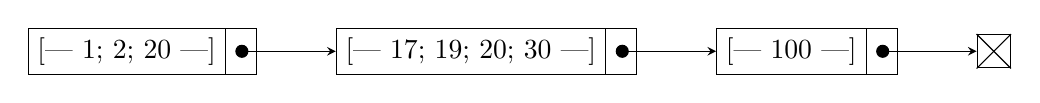
\begin{tikzpicture}[list/.style={rectangle split, rectangle split parts=2,
    	draw, rectangle split horizontal}, >=stealth, start chain]
    
    \node[list,on chain] (A) {[| 1; 2; 20 |]};
    \node[list,on chain] (B) {[| 17; 19; 20; 30 |]};
    \node[list,on chain] (C) {[| 100 |]};
    \node[on chain,draw,inner sep=6pt] (D) {};
    \draw (D.north east) -- (D.south west);
    \draw (D.north west) -- (D.south east);
    \draw[*->] let \p1 = (A.two), \p2 = (A.center) in (\x1,\y2) -- (B);
    \draw[*->] let \p1 = (B.two), \p2 = (B.center) in (\x1,\y2) -- (C);
    \draw[*->] let \p1 = (C.two), \p2 = (C.center) in (\x1,\y2) -- (D);
    \end{tikzpicture}
	\]
	
 \podnaloga Definirajte funkcijo \verb|count: 'a improved_list -> int|, ki vrne število vseh elementov v podanem seznamu.
		
 \podnaloga Definirajte funkcijo, ki vrne i-ti element, če ga seznam vsebuje.
	\begin{verbatim}
    nth: int -> 'a improved_list -> 'a option
	\end{verbatim}
	
 \podnaloga Definirajte funkcijo, ki preveri ali je napreden seznam urejen (predpostavimo, da vsebuje elemente, ki jih lahko primerjamo z \verb|<|). Za vse točke mora funkcija imeti linearno časovno zahtevnost.
	\begin{verbatim}
    is_sorted: 'a improved_list -> bool
	\end{verbatim}
	
 \podnaloga Napišite funkcijo \verb|update: 'a improved_list -> int -> 'a -> 'a improved_list|, ki vrne nov napreden seznam, kjer vrednost na indeksu (drugi argument) nadomesti s podano vrednostjo (tretji argument). Pazite, da pri tem začetni seznam ostane nespremenjen.
	\begin{verbatim}
	# nth (update test 5 (-3)) 5;;
	- : int option = Some (-3)
	# nth test 5;;
	- : int option = Some 20
	\end{verbatim}
	
  \naloga

  \emph{Nalogo lahko rešujete v Pythonu ali OCamlu.}
  
  \podnaloga Mama Franca želijo na balkon širine $n$ postaviti $m$ korit z nageljni širine $l$ (korit, ne nageljnov). Zaradi lažjega zalivanja mora biti med dvema koritoma vsaj za 1 enoto prostora. Mama Franca želijo postaviti vsa korita, jih pa zaradi slabega vida med seboj ne razlikujejo. Primer vseh štirih možnih postavitev pri balkonu širine 9 s tremi koriti širine 2:
  
  \vspace{5mm}
  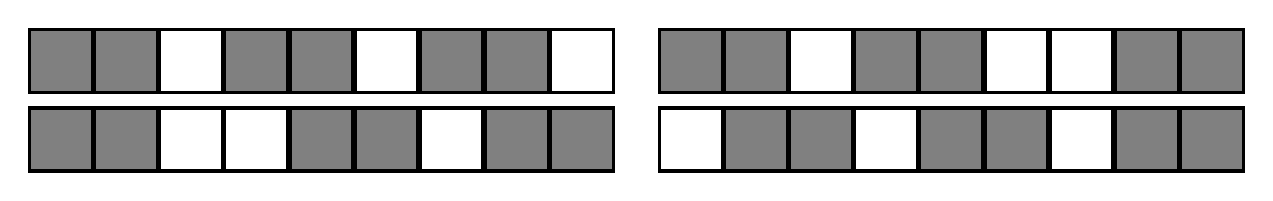
\begin{tikzpicture}
  \tikzstyle{every path}=[very thick]
  \edef\sizetape{0.8cm}
  \tikzstyle{empty}=[draw,minimum size=\sizetape]
  \tikzstyle{filled}=[draw,fill=gray,minimum size=\sizetape]
  \begin{scope}[start chain=1 going right,node distance=-0.15mm]
      \node [on chain=1,filled] {\flower};
      \node [on chain=1,filled] {\flower};
      \node [on chain=1,empty] {};
      \node [on chain=1,filled] {\flower};
      \node [on chain=1,filled] {\flower};
      \node [on chain=1,empty] {};
      \node [on chain=1,filled] {\flower};
      \node [on chain=1,filled] {\flower};
      \node [on chain=1,empty] {};
  \end{scope}
  \begin{scope}[shift={(8cm, 0cm)},start chain=2 going right,node distance=-0.15mm]
      \node [on chain=2,filled] {\flower};
      \node [on chain=2,filled] {\flower};
      \node [on chain=2,empty] {};
      \node [on chain=2,filled] {\flower};
      \node [on chain=2,filled] {\flower};
      \node [on chain=2,empty] {};
      \node [on chain=2,empty] {};
      \node [on chain=2,filled] {\flower};
      \node [on chain=2,filled] {\flower};
  \end{scope}
  \begin{scope}[shift={(0cm,-1cm)}, start chain=3 going right,node distance=-0.15mm]
      \node [on chain=3,filled] {\flower};
      \node [on chain=3,filled] {\flower};
      \node [on chain=3,empty] {};
      \node [on chain=3,empty] {};
      \node [on chain=3,filled] {\flower};
      \node [on chain=3,filled] {\flower};
      \node [on chain=3,empty] {};
      \node [on chain=3,filled] {\flower};
      \node [on chain=3,filled] {\flower};
  \end{scope}
  \begin{scope}[shift={(8cm,-1cm)}, start chain=4 going right,node distance=-0.15mm]
      \node [on chain=4,empty] {};
      \node [on chain=4,filled] {\flower};
      \node [on chain=4,filled] {\flower};
      \node [on chain=4,empty] {};
      \node [on chain=4,filled] {\flower};
      \node [on chain=4,filled] {\flower};
      \node [on chain=4,empty] {};
      \node [on chain=4,filled] {\flower};
      \node [on chain=4,filled] {\flower};
  \end{scope}
  \end{tikzpicture}
	
  \noindent
  Sestavite funkcijo, ki sprejme $n$, $m$ in $l$ ter vrne število vseh različnih postavitev korit za rože na balkon.
 
  \podnaloga Mama Franca so na razprodaji nabrali korita različnih širin. Sestavite funkcijo, ki sprejme širino balkona $n$ in seznam celih števil, ki predstavljajo širine korit, in vrne število različnih postavitev. Pri tem je vrstni red korit določen z vrstnim redom širin v podanem seznamu.
	
\end{document}